Certificador: componente de PPA que "certifica" las demostraciones,
    generando un certificado en deducción natural. Implicó escribir muchos
    meta-teoremas.
    \begin{itemize}
        \item Formalización de muchos teoremas y axiomas: contextos (vale en el prefijo)
        \item Proof y proof steps, simplificación de la interfaz y mapeo de
        comandos a steps
        \item Implementación de cada comando
        \item By y solver para resolver varios. DNF. Extensión con foralls
        consecutivos. Demostración / justificación de que es correcto y completo
        para LP, pero heurístico para LPO (mostrar un caso en el que no funcione)
        \item Descarga de conjunciones
        \item Uso de dneg elim como razonamiento por el absurdo para demostrar
        deMorgan y equivalencias.
    \end{itemize}

En la sección pasada vimos cómo se puede usar PPA para demostrar teoremas. Pero,
¿cómo funciona por detrás? ¿Como asegura la validez lógica de las
demostraciones escritas por el usuario?

\section{Certificados}

Los programas de PPA se \textbf{certifican}, generando una demostración en
deducción natural. ¿Por qué? El lenguaje de PPA es complejo, la implementación
no es trivial. Si se escribe una demostración, para confiar en que es correcta
hay que confiar en la implementación de PPA.

Pero si PPA genera una demostración de bajo nivel, que usa las reglas de un
sistema lógico simple como deducción natural, entonces cualquiera que desconfíe
podría fácilmente escribir un chequeador, o usar uno confiable. Por eso genera
demostraciones en deducción natural, haciendo que cumpla con el \textbf{criterio
de de Bruijn}

\begin{definition}{Criterio de de Bruijn \cite{freek-bruijn}.} Un asistente de
    demostración que satisface que sus demostraciones puedan ser chequeadas por
    un programa independiente, pequeño y confiable se dice que cumple con el
    criterio de de Bruijn.
\end{definition}

El módulo de PPA que \textit{certifica} las demostraciones de alto nivel de PPA
generando una demostración en deducción natural es el \modCertifier{}. Si
bien toda demostración que genere debería ser correcta, para atajar posibles
errores siempre se chequean con el \modChecker{} de DN.


\duda{Para pablo: pero si emite certificados que no corresponden a la demo original y chequean siempre, por ej. siempre el mismo, no estaría mal igual? Tenés que confiar también en la parte que emite el certificado.}

\section{Certificador}

El \modCertifier{} en realidad no genera una sola demostración de deducción
natural, sino que al poder haber más de un teorema en un archivo PPA, este
genera un \textbf{contexto} compuesto por una lista ordenada de
\textbf{hipótesis}. Hay dos tipos

\begin{itemize}
    \item Teoremas: Son fórmulas con demostraciones asociadas.
    \item Axiomas: Son fórmulas que se asumen válidas (pueden ser usadas para
    modelar una teoría)
\end{itemize}

\begin{figure}[H]
    \centering
    \begin{multicols}{2}
        \begin{tabular}{c}
            \lstinputlisting{listings/certifier/two-theorems.ppa}
        \end{tabular}
        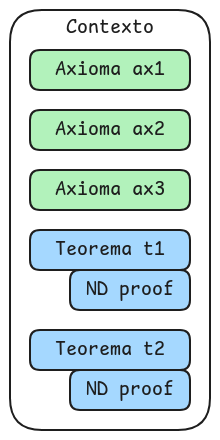
\includegraphics[scale=0.5]{img/ppa-context.png}
    \end{multicols}
    \caption{Contexto resultante de certificar de un programa}
\end{figure}


Por lo tanto, en vez de chequear demostraciones, se chequean contextos: Una
demostración será válida en el \textit{prefijo estricto del contexto} que la
contiene. Es decir, a la hora de chequearla, se deben asumir como ciertas todas
las hipótesis que fueron definidas previamente.

Pero no solo los axiomas y teoremas declarados en el programa se agregan al
contexto. Cada demostración de un teorema tendrá además un \textit{contexto
local} que extiende al anterior, solo en el marco de su demostración. Las
afirmaciones auxiliares que no afectan la tesis (\lstinline{have},
\lstinline{claim}, \lstinline{consider}, etc.) se agregan como teoremas. Por lo
tanto, cuando se citen, se pegan sus demostraciones. Por otro lado, algunos
comandos agregan axiomas, los mismos que en deducción natural agregan fórmulas
al contexto (\lstinline{suppose} y \lstinline{consider}). Es correcto asumir
como ciertas esas hipótesis, porque lo mismo se hará durante el chequeo de la
demostración en deducción natural.

\begin{figure}[H]
    \centering
    \begin{multicols}{2}
        \begin{tabular}{c}
            \lstinputlisting{listings/certifier/local-context.ppa}
        \end{tabular}
        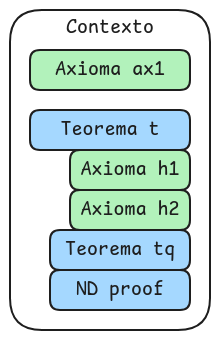
\includegraphics[scale=0.5]{img/ppa-local-context.png}
    \end{multicols}
    \caption{Contexto local}
\end{figure}

\section{Funcionamiento del by}

El \lstinline{by} es el mecanismo principal de demostración en PPA, y el corazón del \modCertifier. Genera
\textbf{automáticamente} una demostración de que una fórmula es consecuencia lógica de
una lista de hipótesis.

Sea $A$ una fórmula. Supongamos que queremos demostrar \lstinline{thus A by h1, ..., hn} y que en el contexto tenemos que las hipótesis $h_i$ corresponden a
fórmulas $\formTwo_i$, con $i \in \{1, ..., n\}, n \in \setNaturals$. Primero
veamos la idea general de la estrategia y luego profundizamos en cada paso.

\begin{itemize}
    \item Queremos demostrar la implicación
    \[
        \formTwo_1 \fAnd \dots \fAnd \formTwo_n \fImp \form
    \]
    \item Razonamos por el absurdo: asumiendo la negación encontramos una contradicción
    \begin{align*}
        \fNot (\formTwo_1 \fAnd \dots \fAnd \formTwo_n \fImp \form)
        &\equiv \fNot (\fNot (\formTwo_1 \fAnd \dots \fAnd \formTwo_n) \fOr \form)\\
        &\equiv \formTwo_1 \fAnd \dots \fAnd \formTwo_n \fAnd \fNot \form
    \end{align*}
    \item Convertimos la fórmula a forma normal disyuntiva (DNF), disyunciones
    de conjunciones de literales. Un literal será un predicado, una negación de
    un literal o una fórmula con cuantificadores.
    \[
        (\formLit^1_{1} \fAnd \dots \fAnd \formLit^1_{n_1})
        \fOr \dots \fOr
        (\formLit^m_{1} \fAnd \dots \fAnd \formLit^m_{n_m})
    \]

    donde $m \in \setNaturals$ es el número de cláusulas, $n_1, \dots, n_m \in
    \setNaturals$ es la cantidad de la cantidad de fórmulas de cada cláusula y
    $\formLit^i_j$ es la $j$-ésima fórmula de la $i$-ésima cláusula.
    \item Buscamos una contradicción refutando cada cláusula (conjunción de literales) individualmente.
    Una cláusula $\formLit_1 \fAnd \dots \fAnd \formLit_n$ será refutable si
    \begin{itemize}
        \item Contiene $\fFalse$
        \item Contiene dos fórmulas opuestas ($\formLit, \fNot \formLit$)
        \item Eliminando existenciales consecutivos y re-convirtiendo a DNF, se
        consigue una refutación ($\fNot \pred(k), \forall \var .\ \pred(x)$)
    \end{itemize}
\end{itemize}

La complejidad del mecanismo no reside solo en tener que realizar todos estos
pasos. El desafío principal fue \textbf{generar la demostración en deducción
natural}. Veamos algunos ejemplos sin generar demostraciones.

\begin{ejemplo}{Ejemplo sin cuantificadores}
    Veamos un ejemplo proposicional.
    \todo{ejemplo sin demo}
\end{ejemplo}

\begin{ejemplo}{Ejemplo con cuantificadores}
    Veamos un ejemplo con cuantificadores.
    \todo{Ejemplo sin demo}
\end{ejemplo}

\subsection{Razonamiento por el absurdo}
\label{ppa-cert:sec:abs-reasoning}

Queremos asumir que no vale la fórmula original, es decir $\fNot (\formTwo_1
\fAnd \dots \fAnd \formTwo_n \fImp \form)$, y llegar a una contradicción. Pero
en la demostración que estamos generando de deducción natural, tenemos que
demostrar $(\formTwo_1 \fAnd \dots \fAnd \formTwo_n \fImp \form)$. ¿Cómo se
puede razonar por el absurdo?

De la misma forma que en la \namedref{nd:sec:admissible-rules} se introduce
\textit{modus tollens} como una regla admisible, para razonar por el absurdo
vamos a usar la \textbf{eliminación de la doble negación}. Es un principio de
razonamiento clásico que es equivalente a LEM.


\begin{theorem}{Eliminiación de la doble negación}
    Sea $\form$ una fórmula cualquiera. Vale \[\fNot \fNot \form \judG \form\]
\end{theorem}
\begin{proof}
    En deducción natural,

    \begin{prooftree}
        \def\defaultHypSeparation{\hskip .1in} % default .2in
        \AxiomC{}
        \LL{\ruleLEM}
        \UnaryInfC{$\fNot \fNot \form \judG \form \fOr \fNot \form$}
        \AxiomC{}
        \RL{\ruleAx}
        \UnaryInfC{\(
            \fNot \fNot \form, \form \judG \form
        \)}
        \AxiomC{}
        \LL{\ruleAx}
        \UnaryInfC{\(
            \fNot \fNot \form, \fNot\form \judG \fNot \fNot \form
        \)}
        \AxiomC{}
        \RL{\ruleAx}
        \UnaryInfC{\(
            \fNot \fNot \form, \fNot\form \judG \fNot \form
        \)}
        \RL{\ruleNotE}
        \BinaryInfC{\(
            \fNot \fNot \form, \fNot \form \judG \form
        \)}
        \RL{\ruleOrE}
        \TrinaryInfC{$\fNot \fNot \form \judG \form$}
    \end{prooftree}
\end{proof}

¿Cómo lo usamos? Introducimos otra regla admisible: \textbf{cut}, que nos
permite ``pegar'' demostraciones entre sí. Si estamos queriendo demostrar
$\form$, y queremos reducirlo a $\formTwo$ que podemos probar, esta regla nos
permite hacerlo.

\begin{theorem}{Cut}. La siguiente regla de inferencia es admisible
\begin{prooftree}
    \AxiomC{$\ctx, \formTwo \judG \form$}
    \AxiomC{$\ctx \judG \formTwo$}
    \RL{\ruleCut}
    \BinaryInfC{$\ctx \judG \form$}
\end{prooftree}
\end{theorem}

\begin{proof}
    En deducción natural. Sean $\someProof_{\formTwo \fImp \form}$ una demostración de $\formTwo
    \judG \form$ y $\someProof_\formTwo$ una demostración de $\formTwo$. La
    regla \ruleCut{} se puede ver como un \textit{macro} que por atrás genera
    la siguiente demostración,
    
    \begin{prooftree}
        \AxiomC{}
        \RL{\ruleImpI}
        \UnaryInfC{$\ctx \judG \formTwo \fImp \form$}
        \AxiomC{$\someProof_\formTwo$}
        \doubleLine
        \UnaryInfC{$\ctx \judG \formTwo$}
        \RL{\ruleImpE}
        \BinaryInfC{$\ctx \judG \form$}
    \end{prooftree}
\end{proof}


¿Y por qué nos permite razonar por el absurdo?

\begin{obs}
    La formulamos como $\fNot \fNot \form \judG \form$ y la usamos con
    \textbf{cut}, pero otra alternativa equivalente, levemente más tediosa para
    generar demostraciones, hubiera sido demostrarla como $\fNot \fNot \form
    \fImp \form$ y ``pegarla'' con \ruleImpE{} directamente.
\end{obs}


\todo{DnegElim como regla admisible, y cómo permite razonar por el absurdo}

\subsection{DNF}

\todo{DNF}

\subsection{Contradicciones}

\todo{contradicciones}

\subsection{Eliminación de universales}

\subsection{Juntando demostraciones}

\todo{Cut como regla admisible}

\subsection{Poder expresivo}

\duda{Está bien decir poder expresivo?}

El solver implementado es \textbf{completo para lógica proposicional}, pero heurístico para lógica de primer orden. Esto es aceptable, puesto que la satisfacibilidad de lógica de primer orden es indecidible \todo{Cita?}, y además el objetivo del trabajo no fue dar el mejor solver, sino dar alguno.

\todo{Citar Hilbert 1950}
\begin{theorem}{El solver es completo para lógica proposicional.}
    \todo{Demo}
\end{theorem}

\subsubsection{Limitaciones}

No puede demostrar por ej.

\todo{ejemplo elim 2 foralls}

\todo{otro ejemplo más burdamente complejo que requiera sat sovler}


\subsection{Unificación}
\label{ppa:sec:unification}

\subsection{Ejemplos completos}

\begin{ejemplo}{Ejemplo sin cuantificadores}
    Veamos un ejemplo proposicional.
    \todo{ejemplo sin demo}
\end{ejemplo}

\begin{ejemplo}{Ejemplo con cuantificadores}
    Veamos un ejemplo con cuantificadores.
    \todo{Ejemplo sin demo}
\end{ejemplo}


\section{Comandos correspondientes a reglas de inferencia}

Como se puede apreciar en \fullref{ppa:tab:inference-rules-to-commands}, la
mayoría de los comandos se corresponden directamente con reglas de inferencia,
por lo que su traducción es más sencilla.

\todo{trad}

\section{Descarga de conjunciones}

\section{Comandos adicionales}

\todo{add}


